% !TEX program = lualatex
% !LW recipe=latexmk (lualatex)
% Compile with LaTeX Workshop/Cursor on save, or run:
%   latexmk -cd -lualatex main.tex

% kao.sty loads hyphenat; pass htt here so \texttt can break across lines.
\PassOptionsToPackage{htt}{hyphenat}

\documentclass[
	fontsize=10pt,
	twoside=false,
	numbers=noenddot,
]{kaobook}

\usepackage[american]{babel}
\usepackage[english=american]{csquotes}

\usepackage[
	citestyle=authoryear-comp,
	bibstyle=authoryear,
	sorting=nyt,
	maxcitenames=2,
	mincitenames=1,
	maxbibnames=99,
	uniquelist=false,
	uniquename=false,
	natbib=true,
]{kaobiblio}
\addbibresource{main.bib}
\let\cite=\parencite

\usepackage[framed=true]{kaotheorems}
\usepackage{kaorefs}

\usepackage{booktabs}
\usepackage{svg}
\usepackage{tabularx}
\usepackage{tikz}
\usetikzlibrary{arrows.meta,positioning}

% Draft builds skip external image rendering and mark overfull boxes. Compile
% main-draft.tex for this mode; use main.tex for final output.
\ifdefined\thesisdraft
	\setkeys{Gin}{draft}
	\overfullrule=5pt
\fi

\usepackage{iftex}
\ifPDFTeX
	\usepackage{libertine}
	\newcommand*{\headingfont}{\fontfamily{LinuxBiolinumT-LF}\selectfont}
\else
	\usepackage{fontspec}
	\IfFontExistsTF{Linux Biolinum O}{%
		\newfontfamily\biolinumfont{Linux Biolinum O}[
			Ligatures=TeX,
			BoldFont={Linux Biolinum O Bold},
			ItalicFont={Linux Biolinum O Italic},
		]%
	}{%
		\newfontfamily\biolinumfont{Latin Modern Roman}%
	}
	\newcommand*{\headingfont}{\biolinumfont}
\fi

\addtokomafont{part}{\headingfont}
\addtokomafont{partentry}{\headingfont}
\addtokomafont{chapter}{\headingfont}
\addtokomafont{chapterentry}{\headingfont}
\addtokomafont{section}{\headingfont}
\addtokomafont{subsection}{\headingfont}
\addtokomafont{subsubsection}{\headingfont}

\graphicspath{{figs/}}
\makeindex[columns=3, title=Alphabetical Index, intoc]
% Uncomment when using glossary or nomenclature entries.
% \makeglossaries
% \makenomenclature

% Shared thesis commands.

\DeclareMathOperator*{\Eop}{\mathbb{E}}
\DeclareMathOperator*{\Varop}{\mathbb{V}}
\DeclareMathOperator*{\Argmax}{arg\,max}
\DeclareMathOperator*{\Argmin}{arg\,min}

\NewDocumentCommand{\E}{o m}{%
  \IfNoValueTF{#1}{%
    \Eop\!\left[#2\right]%
  }{%
    \Eop_{\substack{#1}}\!\left[#2\right]%
  }%
}
\NewDocumentCommand{\Var}{o m}{%
  \IfNoValueTF{#1}{%
    \Varop\!\left[#2\right]%
  }{%
    \Varop_{\substack{#1}}\!\left[#2\right]%
  }%
}

\newcommand{\R}{\mathbb{R}}
\newcommand{\calD}{\mathcal{D}}
\newcommand{\calL}{\mathcal{L}}

% A simple placeholder for examples. Replace this with \includegraphics when
% using real figure files.
\newcommand{\placeholderfigure}[2][\linewidth]{%
  \begin{tikzpicture}
    \node[
      draw=black!35,
      fill=black!3,
      rounded corners=2pt,
      minimum width=#1,
      minimum height=#2,
      align=center,
      inner sep=0pt
    ] {Example figure\\\texttt{\string\includegraphics}};
  \end{tikzpicture}%
}


% For faster chapter-focused passes, uncomment and keep only the chapters you
% are actively editing. Compile once without \includeonly before final checks.
% \includeonly{chapters/introduction,chapters/examples}

\begin{document}

\subject{Master's Thesis}
\title[Short Thesis Title]{Thesis Title\\[-0.35em]with Manual Line Breaks\\[0.15em]for the Title Page}
\author{Author Name}
\date{\today}
\newcommand{\thesisadvisors}{%
	\normalsize Advisor Name\\
	\normalsize Co-advisor Name\\
	\normalsize Prof.\ Dr.\ Supervisor Name
}

\makeatletter
\renewcommand{\maketitle}{
\begin{titlepage}
	\begin{minipage}[t]{\textwidth}
		\newcommand{\titleETHLogoHeight}{0.68cm}
		\newcommand{\titleLabLogoHeight}{0.95cm}
		\newcommand{\titleLogoGap}{0.32cm}
		\makebox[\textwidth]{%
			\raisebox{-0.5\height}{\includesvg[height=\titleETHLogoHeight]{eth_logo_kurz_pos.svg}}%
			\hfill
			\raisebox{-0.5\height}{\includesvg[height=\titleLabLogoHeight]{spylab_logo.svg}}%
			\hspace{\titleLogoGap}%
			\raisebox{-0.5\height}{
\includegraphics[height=\titleLabLogoHeight]{las_logo.png}}%
		}
	\end{minipage}
	\vspace*{5.35cm}
	\begin{center}
		{\headingfont\LARGE\textbf{\@subject}}\\[1cm]
		{\headingfont\fontsize{28}{32}\selectfont\textbf{\@title}}\\[1.4cm]
		\large\@author\\
		\large\@date
	\end{center}
	\vfill
	\begin{center}
		\normalsize\textbf{Advisors}\\
		\thesisadvisors
	\end{center}
	\vspace*{-0.3cm}
\end{titlepage}
}
\makeatother

\frontmatter
\maketitle

% !TEX root = ../main.tex

\chapter*{Abstract}
\addcontentsline{toc}{chapter}{Abstract}

This template is a compact starting point for a thesis using the local
\texttt{kaobook} setup. It keeps the structure of a complete project: front
matter, parts, chapters, a bibliography, and appendices. The example chapters
show the supported figure and table layouts without carrying over project
specific thesis content.

% !TEX root = ../main.tex

\chapter*{Acknowledgements}
\addcontentsline{toc}{chapter}{Acknowledgements}

Thank the people, groups, or institutions that supported the thesis. Delete
this page if your program does not require acknowledgements.


\begingroup
\etocclasstocstyle
\etocstandardlines
\setcounter{tocdepth}{\sectiontocdepth}
\tableofcontents
% \listoffigures
% \listoftables
\endgroup

\mainmatter
\setchapterstyle{kao}

\part{Thesis Body}
% !TEX root = ../main.tex

\chapter{Introduction}
\label{ch:introduction}

Start each chapter in its own file and include it from \texttt{main.tex}. This
keeps the root file focused on document structure and package configuration.

\section{Cross References}
\label{sec:cross-references}

Use labels for chapters, sections, figures, tables, equations, and appendix
material. For example, chapter~\ref{ch:examples} shows the figure and table
patterns, while appendix~\ref{app:additional-material} contains supporting
material. Citations are handled by \texttt{biblatex}; here is a textual citation
with \textcite{knuth1984texbook} and a parenthetical citation \cite{lamport1994latex}.

\begin{definition}[Reusable command]
A reusable command is a short macro in \texttt{macros.tex} that captures
notation used throughout the thesis.
\end{definition}

For example, \(\E[x \sim p]{x^2}\) is defined once in \texttt{macros.tex} and
can then be used consistently in every chapter.

% !TEX root = ../main.tex

\chapter{Figures and Tables}
\label{ch:examples}

This chapter is intentionally practical: it contains the small and full-width
float patterns that most thesis projects need. The figures use copied example
images from the source thesis so the template shows the actual supported image
workflow.

\section{Figures}
\label{sec:figures}

\begin{figure}
	\centering
	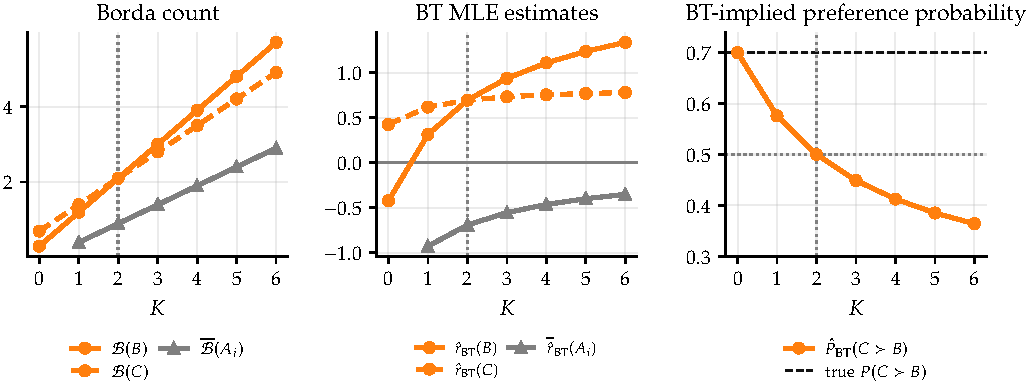
\includegraphics[width=0.86\linewidth]{tabular/social_choice_borda_bt.pdf}
	\caption{A regular figure. Its caption sits in the margin in the standard
	kaobook layout. Use this for figures that fit naturally in the text column.}
	\label{fig:regular-figure}
\end{figure}

Reference regular figures with \texttt{\string\ref}: Figure~\ref{fig:regular-figure}
is a text-column float. With an image file, use \texttt{\string\includegraphics}
with a width such as \texttt{\string\textwidth} or \texttt{0.8\string\linewidth}.

\begin{figure*}
	\centering
	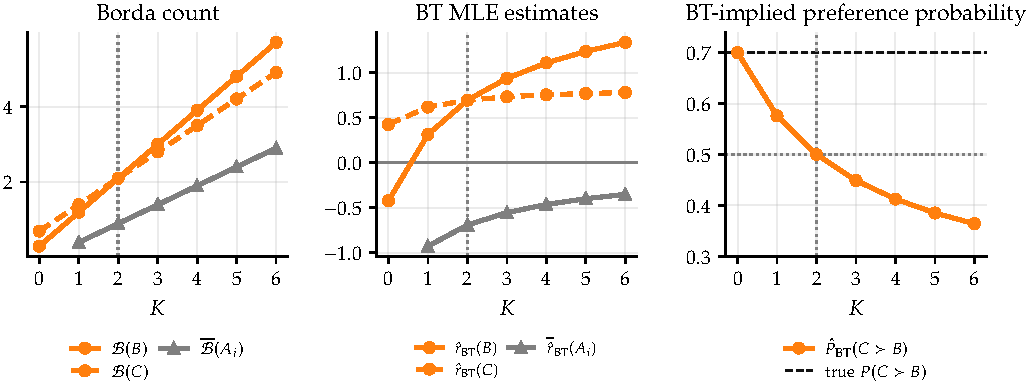
\includegraphics[width=0.92\linewidth]{tabular/social_choice_borda_bt.pdf}
	\caption{A full-width figure. Use \texttt{figure*} when the content needs
	the text column and the margin together.}
	\label{fig:full-width-figure}
\end{figure*}

Figure~\ref{fig:full-width-figure} uses the full available page width. This is
useful for multi-panel figures, dense plots, or diagrams with long labels.

\section{Tables}
\label{sec:tables}

\begin{table}
	\centering
	\begin{tabular}{lrr}
		\toprule
		Method & Score & Time \\
		\midrule
		Baseline & 0.71 & 12.4 \\
		Proposed & 0.83 & 10.9 \\
		\bottomrule
	\end{tabular}
	\caption{A regular table for compact results. Keep column names short and
	put details in the caption or surrounding text.}
	\label{tab:regular-table}
\end{table}

Table~\ref{tab:regular-table} is a normal text-column table.

\begin{table*}
	\centering
	\small
	\begin{tabularx}{0.95\linewidth}{lrrrrX}
		\toprule
		Setting & Train & Valid & Test & Runtime & Notes \\
		\midrule
		Small & 100 & 20 & 20 & 1.2 min & Useful for smoke tests and examples. \\
		Medium & 1000 & 200 & 200 & 8.4 min & Fits comfortably in a wider table. \\
		Large & 10000 & 2000 & 2000 & 51.0 min & Use wide tables for many columns or longer notes. \\
		\bottomrule
	\end{tabularx}
	\caption{A full-width table. Use \texttt{table*} for wide result summaries
	or tables with explanatory columns.}
	\label{tab:full-width-table}
\end{table*}

Table~\ref{tab:full-width-table} demonstrates the wide-table layout and
\texttt{tabularx} for a flexible notes column.


\part{Results}
% !TEX root = ../main.tex

\chapter{Results}
\label{ch:results}

Use this chapter for the core findings. A short equation can stay in the text
column:
\[
	\calL(\theta) = \E[(x,y) \sim \calD]{\ell(f_\theta(x), y)}.
\]

For equations that need more horizontal room, use the kaobook
\texttt{wideequation} environment:
\begin{wideequation}
	\Argmin_{\theta \in \R^d}
	\E[(x,y) \sim \calD]{\ell(f_\theta(x), y)}
	+ \lambda \lVert \theta \rVert_2^2.
\end{wideequation}

Discuss what the result means, then point to the supporting details in
appendix~\ref{app:additional-material}.

% !TEX root = ../main.tex

\chapter{Conclusion}
\label{ch:conclusion}

Summarize the thesis contribution, limitations, and the most direct next steps.
Keep the conclusion self-contained enough that a reader can understand what was
shown after skimming the introduction and results.


\printbibliography

\appendix
\part{Appendix}
% !TEX root = ../main.tex

\chapter{Additional Material}
\label{app:additional-material}

Appendices are normal chapters after \texttt{\string\appendix}; LaTeX changes
their numbering automatically. Put derivations, extended tables, extra figures,
questionnaires, or implementation details here.

\section{Derivation Sketch}

This section shows where detailed derivations can live. The main text can refer
to this material without interrupting the thesis narrative.

\begin{equation}
	\Var{X} = \E{X^2} - \E{X}^2.
\end{equation}


% Optional supporting lists. Uncomment when used.
% \printnomenclature
% \printglossary[title=Special Terms, toctitle=List of Terms]
% \printglossary[type=\acronymtype,title=Abbreviations, toctitle=List of Abbreviations]
% \printindex

\end{document}
